\chapter{Planejamento do projeto}

Nesta seção será abordado um cronograma que a equipe se baseou para a realização das atividades até a data de entrega deste documento. Nesse cronograma estão destacadas as datas de entrega das atividades e os responsáveis por cada uma delas, isso torna mais fácil o contato com a pessoa que realizou a atividade caso a mesma precise de alguns ajustes.

\section{Cronograma}

	O cronograma a seguir mostra quais as atividades foram executadas pela equipe, além de quais recursos humanos e de tempo foram alocados para execução dos mesmos. Foi utilizado o Gantter que é uma ferramenta para gestão de projetos open-source.

	\begin{figure}[!htpb]
	\centering
	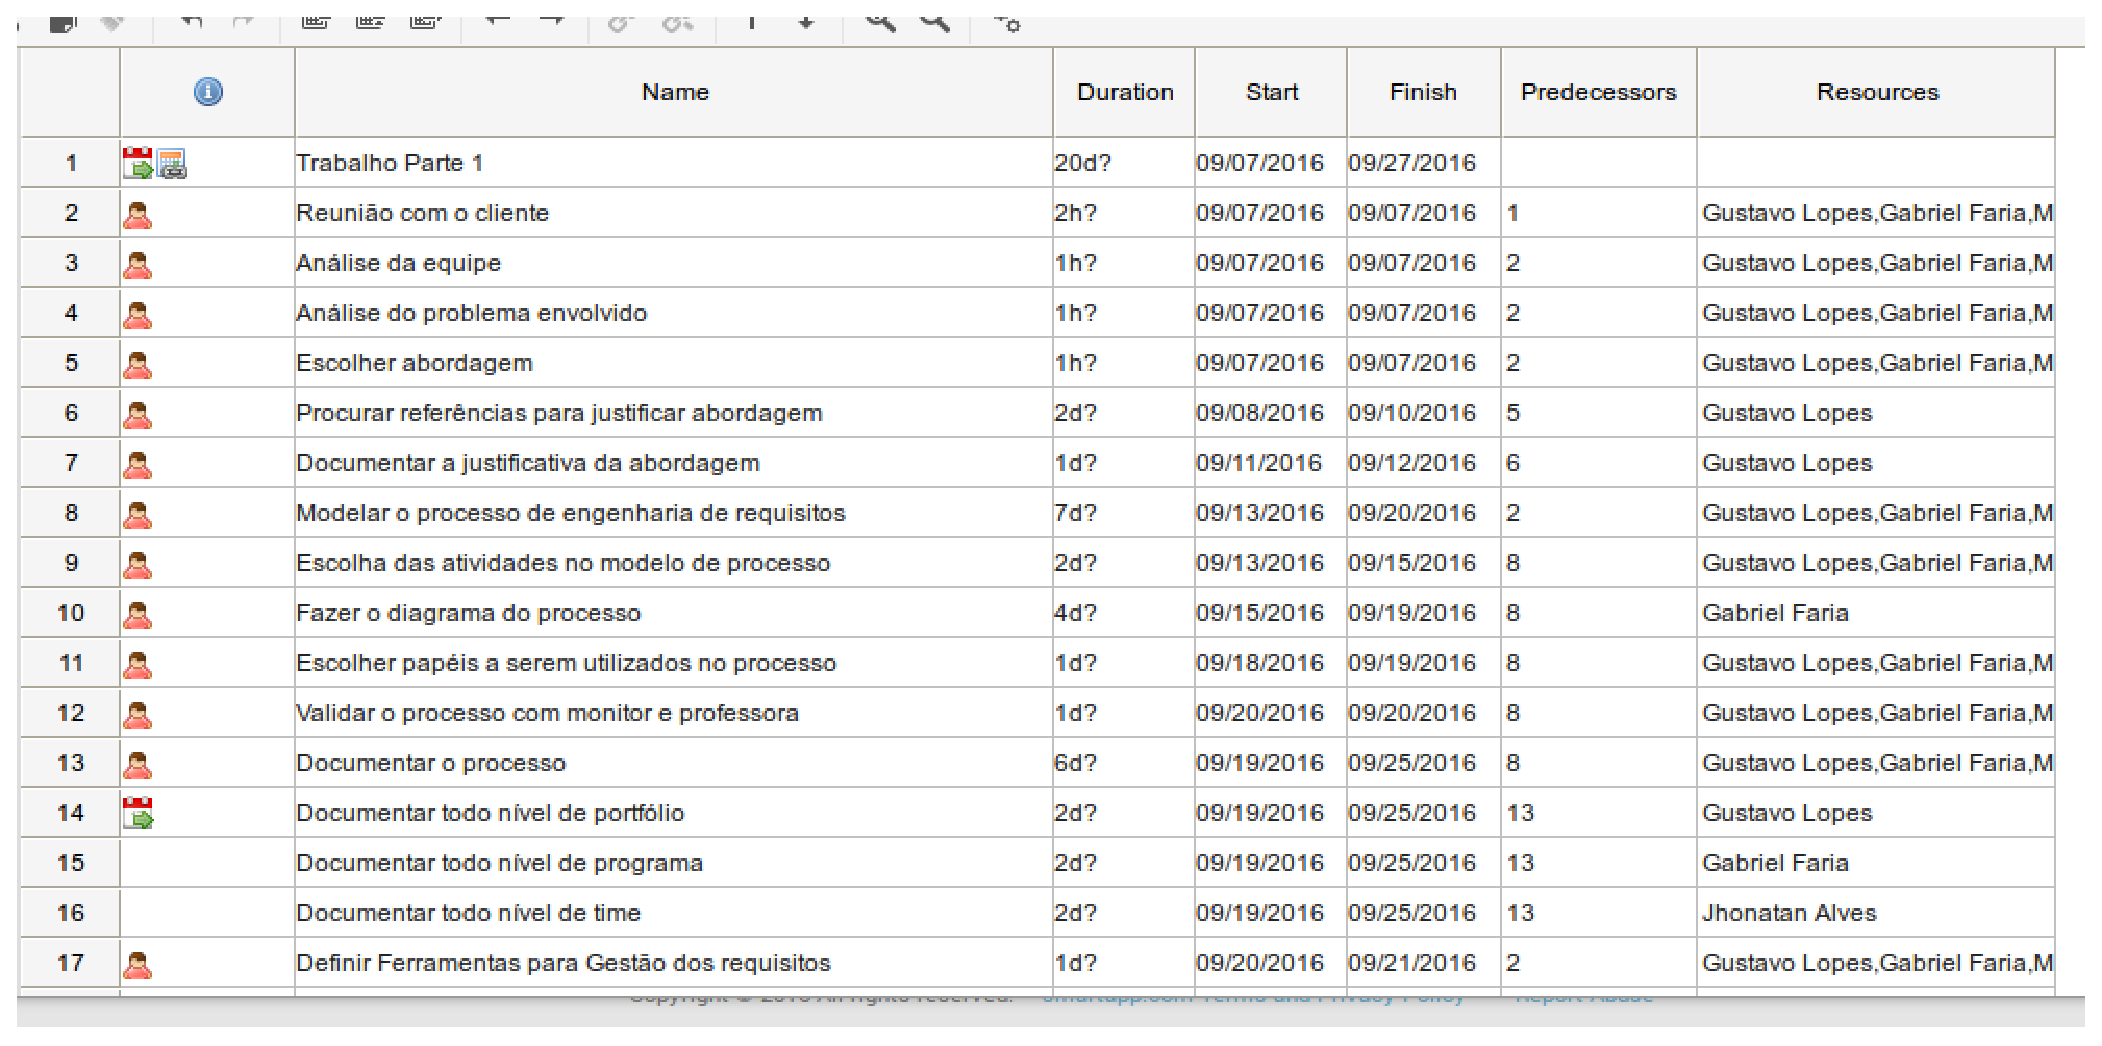
\includegraphics[scale=0.4]{figuras/cronograma/parte1}
	\caption{Exibição do cronograma e suas atividades e durações}
	\end{figure}

	\begin{figure}[!htpb]
	\centering
	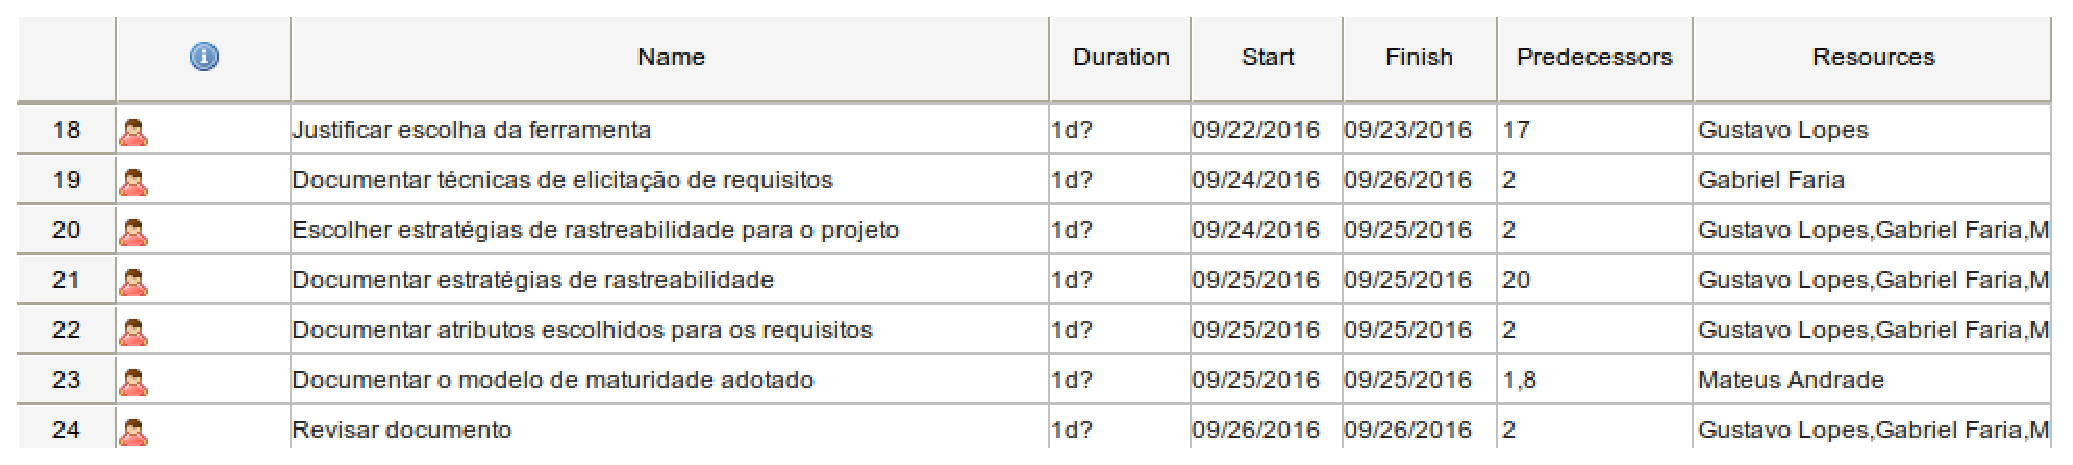
\includegraphics[scale=0.4]{figuras/cronograma/parte2}
	\caption{Parte 2 do cronograma}
	\end{figure}
